\documentclass[12pt]{article}


%For stacking text, used here in autosegmental diagrams
\usepackage{stackengine}

%To combine rows in tables
\usepackage{multirow}

%geometry helps manage margins, among other things.
\usepackage[margin=1in]{geometry}

%Gives some extra formatting options, e.g. underlining/strikeout
\usepackage{ulem}

%For putting links into papers, also helps make cross-references in the paper smart references
\usepackage[colorlinks = true,
            linkcolor = blue,
            urlcolor  = blue,
            citecolor = blue,
            anchorcolor = blue]{hyperref} %smarter cross-references, these options turn links blue

%Use package/command below to create a double-spaced document, if you want one. Uncomment BOTH the package and the command (\doublespacing) to create a doublespaced document, or leave them as is to have a single-spaced document.
%\usepackage{setspace}
%\doublespacing 

%paragraph formatting
\usepackage[parfill]{parskip}
\setlength{\parskip}{5pt} %plus 1 minus 1}
\setlength{\parindent}{30pt}
\usepackage{titlesec}

%use for special OT tableaux symbols like bomb and sad face. must be loaded early on because it doesn't play well with some other packages
\usepackage{fourier-orns}

%Basic math symbols 
\usepackage{pifont}
\usepackage{amssymb}

%%%Gives shortcuts for glossing. The use of this package is NOT explained in the Quick Reference Guide, but the documentation is on CTAN for those that are interested. MJKD finds it handy for glossing. (https://ctan.org/pkg/leipzig?lang=en)
\usepackage{leipzig}

%Tables
\usepackage{caption} %For table captions
\usepackage{booktabs} %helps format tables

%For citations and bibliography - as of 9.1.2019 we don't explain citations in this Quick Reference Guide, but Pedro Martin's tutorial does (see links in the Guide).
\usepackage{natbib}

%For OT-style tableaux
\usepackage{ot-tableau}

%Fonts
\usepackage[no-math]{fontspec} %This allows you to enter (via an IPA kayboard) IPA fonts and other symbols directly into LaTeX. Requires a particular setyp, see below.
\usepackage{libertine} %A font that actually contains many IPA symbols. This is the font you see in the preview to the right.

%to use these fonts, be sure that your typesetting engine is set to "XeLaTeX." In Overleaf, go to the Menu link on the top left (by the Overleaf icon), and under Settings be sure that the Compiler is set to "XeLaTeX." If you accessed this document via the Overleaf Pomona Linguistics template, all of this was already done for you.

%The Pomona Linguistics Paper Template in Overleaf is already set up for this, but you may run into this problem if you start building your own documents.

%highlights text with \hl{text}
\usepackage{color, soul}

%Drawing Syntax Trees
\usepackage[linguistics]{forest}

%This specifies some formatting for the forest trees to make them nicer to look at
\forestset{
  nice nodes/.style={
    for tree={
      inner sep=0pt,
      fit=band,
    },
  },
  default preamble=nice nodes,
}

%% For numbered and glossed examples %%
\usepackage{gb4e}



%Changes the \maketitle command to be smaller and take up less space on a page. 
\makeatletter         
\def\@maketitle{   % custom maketitle 
\noindent {\Large \bfseries \color{black} \@title}  \\ \hrule \noindent \@author \\ \@date  
}

%The code below will draw a circle around a piece of text. This is very useful for drawing attention to a word in a data example. use the command \circled{text} where the argument (`text' here) is what you want to be circled. This is illustrated in the Quick Reference Guide and the Paper Template.

\usepackage{tikz}

\newcommand{\circled}[1]{\begin{tikzpicture}[baseline=(word.base)]
\node[draw, rounded corners, text height=8pt, text depth=2pt, inner sep=2pt, outer sep=0pt, use as bounding box] (word) {#1};
\end{tikzpicture}
}


%%%%%%%%%%%%%%%%%%%%%%%%%%%%%%%%%%%%%%%%%%%%%%%%%%%%%%%%%%%%
%%%%%%%%%%%%%%%%%%%%%%%%%%%%%%%%%%%%%%%%%%%%%%%%%%%%%%%%%%%%

% Useful Ling Shortcuts

\RequirePackage{leipzig}
%\RequirePackage{mathtools} % for \mathrlap

% % % Shortcuts  (borrowed from JZ, I'm still unsure exactly what xspace requires)
\RequirePackage{xspace}
\xspaceaddexceptions{]\}}

%This makes the \emptyset command be a nicer one
\let\oldemptyset\emptyset
\let\emptyset\varnothing
\newcommand{\nothing}{$\emptyset$}

%Not all of these are explained in the Quick Reference Guide, but they are here bc they are relevant to some of our students.
\newcommand{\1}{\rlap{$'$}\xspace}
\newcommand{\0}{\rlap{\textsuperscript{$ˆ{\circ}$}}\xspace}
\newcommand{\Lb}[1]{$\text{[}_{\text{#1}}$ } %A more convenient left bracket
\newcommand{\Rb}[1]{$\text{]}_{\text{#1}}$ } %A more convenient left bracket
\newcommand{\gap}{\underline{\hspace{1.2em}}}
\newcommand{\vP}{\emph{v}P}
\newcommand{\lilv}{\emph{v}}
\newcommand{\Abar}{A$'$-} %A more convenient A-bar notation
\newcommand{\ph}{$\varphi$\xspace} %A more convenient phi
\newcommand{\pro}{\emph{pro}\xspace}
\newcommand{\subs}[1]{\textsubscript{#1}} %A more convenient subscript
%\newcommand{\hd}{$^{\circ}$\xspace} %Symbol for printing head / degree symbol
\newcommand{\spells}{$\Longleftrightarrow$} %spellout arrow for morph spellout rules
\newcommand{\tr}[1]{\textit{t}\textsubscript{\textit{#1}}} %easy traces with subscript
\newcommand{\supers}[1]{\textsuperscript{#1}}

% Abbreviations for glossing, based on Leipzig
\newleipzig{hab}{hab}{habitual}
\newleipzig{rem}{rem}{remote}
\newleipzig{sm}{sm}{subject marker}
\newleipzig{t}{t}{tense}
\newleipzig{aa}{aa}{anti-agreement}
\newleipzig{pron}{pron}{pronoun}
\newleipzig{rec}{rec}{recent}
\newleipzig{om}{om}{object marker}
%\newleipzig{ipfv}{ipfv}{imperfective}
\newleipzig{asp}{asp}{aspect}
\newleipzig{lk}{lk}{linker}
\newleipzig{pcl}{pcl}{particle}
\newleipzig{stat}{stat}{stative}
\newleipzig{ints}{ints}{intensive}
\newleipzig{ascl}{ascl}{assertive subject clitic}
\newleipzig{nascl}{nascl}{non-assertive subject clitic}
\newleipzig{ta}{ta}{tense and/or aspect}
\newleipzig{assoc}{assoc}{associative marker}
\newleipzig{hon}{hon}{honorific}
%\newleipzig{whprt}{wh}{\wh particle}
\newleipzig{sa}{sa}{subject agreement}
\newleipzig{conj}{conj}{conjunction}
%\newleipzig{loc}{loc}{locative}
\newleipzig{expl}{expl}{expletive}
\newleipzig{rcm}{rcm}{reciprocal marker}
\newleipzig{pers}{pers}{persistive}
%\newleipzig{}{}{} %this is just to copy for when I want to add more

%%%%%%%%%%%%%%%%%%%%%%%%%%%%%%%%%%%%%%%%%%%%%%%%%%%%%%%%%%%%
%%%%%%%%%%%%%%%%%%%%%%%%%%%%%%%%%%%%%%%%%%%%%%%%%%%%%%%%%%%%

%A couple of packages that seemed to prefer being called toward the end of the preamble

%This package provides macros for typesetting SPE-style phonological rules.
\usepackage{phonrule}

%For using Greek letters outside of math mode.
\usepackage{textgreek}


%Random, lets us use the XeLaTeX logo. Not important to the template at all.
\usepackage{metalogo}

\usepackage{tikz} 
\usepackage{caption}
\usepackage{caption}
\usepackage{subcaption}

%%%%%%%%%%%%
%% This is the end of the PREAMBLE
%%%%%%%%%%%


\usepackage{floatrow}
\usepackage{alltt}
\usepackage{xcolor}

% Table float box with bottom caption, box width adjusted to content
\newfloatcommand{capbtabbox}{table}[][\FBwidth]

\usepackage{blindtext}
\renewcommand*{\thesection}{\Roman{section}}
\setlength\parindent{0pt}


\renewenvironment{table}%
  {\renewcommand\familydefault\sfdefault
   \@float{table}}
  {\end@float}
\makeatother

\usepackage{booktabs} \newcommand{\ra}[1]{\renewcommand{\arraystretch}{#1}}
\newcommand{\code}[1]{\colorbox{gray!18}{\texttt{#1}}}
\renewcommand{\labelitemi}{\raisebox{.25\height}{\tiny$\blacksquare$}}

\newcommand{\JMUTitle}[9]{

  \thispagestyle{empty}
  {\parindent0cm
  \rule{\linewidth}{.7ex}}
  
  \begin{center}
    \vspace*{\stretch{1}}
    \sffamily\bfseries\Huge
    #1\\
    \vspace*{\stretch{1}}
    \sffamily\bfseries\large
    #2
    \vspace*{\stretch{1}}
  \end{center}
  \rule{\linewidth}{.7ex}

  \vspace*{\stretch{1}}
  \begin{center}
    
\includegraphics{LogoUBFC.jpg} \\
    \vspace*{\stretch{1}}
    \Large Neha Binish  \\
    \vspace*{\stretch{1}}
    \Large Supervisor:  Ludovic Martin-Gondre  \\

    \vspace*{\stretch{2}}
    \large Master of Computational Physics\\
    \large Physics department\\
    \large Université Bourgogne Franche-Comté\\
    \vspace*{\stretch{1}}
    
  \end{center}
}

\begin{document}

\JMUTitle
      {Numerical Project - FORTRAN}
      {Building of a multidimensional potential energy surface applied to
       the gas/surface reactivity}                       

      
      { }  
      {Besançon  2021}                         
      
      { }                              
      { }                         
      
  \clearpage

\tableofcontents
\clearpage 

\section{PROGRESS OF THE PROJECT}
\par\noindent\rule{\textwidth}{0.4pt}

\textbf{Version}: Alpha version 

\textbf{End of Development Date}: 5\textsuperscript{th} March, 2021

\textbf{Programming Language}: FORTRAN90

\textbf{Format}: Source code
\par\noindent\rule{\textwidth}{0.4pt}

\section{LIST OF FILES}
\par\noindent\rule{\textwidth}{0.4pt}
In order to increase readability, the project is made of several files. The curve fitting and the plots are made using python3, whereas the development of the LEPS potential energy surfaces is done using FORTRAN90. 

{\fontsize{10}{6}\textbf{\textcolor{red}{\texttt{fit.py}}}}: Non - linear curve fitting in Python3

{\fontsize{10}{6}\textbf{\textcolor{red}{\texttt{main.f90}}}} (main program) : Building of the LEPS potentials

{\fontsize{10}{6}\textbf{\textcolor{red}{\texttt{sub.f90}}}}: Modules required to generate 3D-PES scripts and 1-D cuts

{\fontsize{10}{6}\textbf{\textcolor{red}{\texttt{savearray.py}}}}: Python Program to read text files and save as arrays.

{\fontsize{10}{6}\textbf{\textcolor{red}{\texttt{3dplot.py}}}}: Plot of the 3-D-PES script

{\fontsize{10}{6}\textbf{\textcolor{red}{\texttt{error.f90}}}} : Program for Error Analysis

{\fontsize{10}{6}\textbf{\textcolor{red}{\texttt{min.f90}}}} :  Program to find the Global Minimum


\section{FUNCTIONAL SPECIFICATIONS}
\par\noindent\rule{\textwidth}{0.4pt}

\subsection{Goal of the Program}

The goal of this project is to build multidimensional potential energy surface to describe N-N\textsubscript{2} interacting with the tungsten surfaces, specifically for the crystallographic plane W(100).

The potential energy surfaces are build using an analytical model called the LEPS (London Eyring Polanyi Sato) model. Initially, the required potential energies are extracted from the numerical model called the CRP model that has been provided for the N\textsubscript{{2}}/W(100) system. These potential energies are then used to carry out a curve fitting to obtain the various parameters of the LEPS model. 

The CRP-PES also behaves as a reference model that serves to compare the quality of the LEPS-PES generated. The attained version of the program builds a 3D-PES for the N/W(100) atom-surface
\subsection{ Input Data }

This program uses several piece of data that can be set by the user to extract the required potential. The potential energies extracted are saved as text file in the folder outputs in the format:
\begin{center}
\textbf{<symmetry-name><crp/leps>.txt}  
\end{center} 

All the files required for the execution of the program are saved in the folder {\fontsize{10}{6}\code{files}}. These files can be loaded into the programs for trial runs. 

The following parameters are input by the user to extract the required potential at different symmetry sites.
\begin{table*}[h!]\centering
\ra{1.3}
\resizebox{\linewidth}{!}{%
\begin{tabular}{ccc}\toprule
\textbf{Parameters}  & \textbf{Description} & \textbf{Type}\\\toprule
\multicolumn{3}{c}{\textbf{Input data for extracting potential energies from CRP-PES}}\\ \hline
xa & Location on the x-axis in units of delta & Double Precision\\
ya & Location on the y-axis in units of delta & Double Precision\\
Zmin & Beginning of the location of the grid on z-axis & Double Precision \\
Zmax & End of the location of the grid on z-axis & Double Precision\\
Ntot & Total number of potential energies and distances extracted & Integer\\\hline
\multicolumn{3}{c}{\textbf{Input data for main program}}\\ \hline
delta ($\delta) $ & the unit cell parameter & Real - Double Precision\\
N & Total number of points in the grid & Integer \\
\midrule
Xtop & x-axis location of TOP symmetry site (in units of delta) & Real - Double Precision\\
Ytop & y-axis location of TOP symmetry site (in units of delta) & Real - Double Precision \\
Xhollow & x-axis location of HOLLOW symmetry site (in units of delta) & Real - Double Precision\\
Yhollow & y-axis location of HOLLOW symmetry site (in units of delta) & Real - Double Precision \\
Xbridge & x-axis location of BRIDGE symmetry site (in units of delta) & Real - Double Precision\\
Ybridge & y-axis location of BRIDGE symmetry site (in units of delta) & Real - Double Precision \\
\midrule
Dtop & Morse potential parameter - D for high symmetry site - TOP & Real - Double Precision\\
Dhollow & Morse potential parameter - D for high symmetry site - HOLLOW & Real - Double Precision\\
Dbridge & Morse potential parameter - D for high symmetry site - BRIDGE & Real - Double Precision\\
\midrule
alphatop & Morse potential parameter - $\alpha$ for high symmetry site - TOP & Real - Double Precision\\
alphahollow & Morse potential parameter - $\alpha$ for high symmetry site - HOLLOW & Real - Double Precision\\
alphabridge & Morse potential parameter - $\alpha$ for high symmetry site - BRIDGE & Real - Double Precision\\
\midrule
reqtop & Morse potential parameter - $r^{eq}$ for high symmetry site - TOP & Real - Double Precision\\
reqhollow & Morse potential parameter - $r^{eq}$  for high symmetry site - HOLLOW & Real - Double Precision\\
reqbridge & Morse potential parameter - $r^{eq}$  for high symmetry site - BRIDGE & Real - Double Precision\\\hline
\end{tabular}}
\caption{Input data}
\end{table*} 



\subsection{ Output Data }

In the alpha version, the program outputs several plots of 1-D cuts for different symmetry sites. These plots are saved in the folder figures in the following format:
\begin{center}
\textbf{<symmetry-name>.png}  

\textbf{<1d/3d><symmetry-name>.png}

\end{center}
The potential energies extracted from CRP-PES and LEPS-PES, are saved as text files in the folder outputs and later these text files are also used as inputs in the given format:
\begin{center}
\textbf{<p/z><crp/pes>\_<symmetry-name>.txt}  
\end{center}                       
The figures generated are stored in the folder {\fontsize{10}{6}\code{figures}}.

In addition to this, the program also computes the following parameters:

\begin{table*}[h!]\centering
\ra{1.3}
\resizebox{\linewidth}{!}{%
\begin{tabular}{ccc}\toprule
\textbf{Parameters}  & \textbf{Description} & \textbf{Type}\\\toprule
Coeff\_D & Fourier coefficients of the Morse potential parameter - D & Real - Double Precision - size(3,1)\\
Coeff\_alpha & Fourier coefficients of the Morse potential parameter - $\alpha$  & Real - Double Precision - size(3,1)\\
Coeff\_req & Fourier coefficients of the Morse potential parameter - $r^{eq}$ & Real - Double Precision - size(3,1)\\
M\_error & Mean absolute error & Real - Double Precision\\
REL\_error& Relative error & Real - Double Precision\\
CRP\_min & Global minimum of the CRP-PES & Real - Double Precision\\
LEPS\_min & Global minimum of the LEPS-PES & Real - Double Precision\\
\hline
\end{tabular}}
\caption{Output data}
\end{table*} 

\subsection{Specific Conditions of Use}
\vspace{5mm}
\begin{itemize}

    \item The README file contain instructions on how to generate potential energies from the CRP-PES scripts (energies are in eV and distances are in \AA). However, the user must previously generate the executable file  {\fontsize{10}{6}\code{textat.exe}}, without which the script fails to run
    
    \item On extracting the CRP-PES potentials and distances at different positions and symmetry, curve fitting was attempted. It was found that when the values from zmin = 0 was included, curve fitting using python polyfit was not possible as the function was unable to find the right parameters for the fit due to the high fluctuation of the potential around zmin = 0, when it tends to infinity. 
    
     \item Hence, for a good for using polyfit function in python 3, the first few values of the potential was cut off for specific symmetry sites and the potentials are  extracted from distances zmin = 0.5.
    
    \item Moreover, for error optimization, the user is required to choose the right range of values on the z-axis over which the potential energies are extracted. 

    \item The user is also required to have all the modules pre-loaded and compiled.
    
    \item In order to run a trial with the existing text files, it is necessary to include the path of these files and the user also has to take care not to rewrite the files or false results could be produced. 
    
\end{itemize}


\section{INTERNAL FUNCTIONING OF THE PROGRAM}
\par\noindent\rule{\textwidth}{0.4pt}

\subsection{ Physical Model}

\vspace{5mm}
\subsubsection{CRP-PES}
To interpret and compare the LEPS potential, it is necessary to extract the potentials energies from the CRP-PES for various positions of N onto W(100) surface. 

We refer to the README file in order to generate potential energies from the CRP-PES scripts provided. The output data consisting of potential energies (in eV) and the corresponding distances (in \AA) are extracted for different symmetry sites. For this particular project - the data was extracted for the following points -
\begin{table*}[h!]\centering
\ra{1.3}
\resizebox{\linewidth}{!}{%
\begin{tabular}{cccccc}\toprule
\textbf{Symmetry Sites}  & \textbf{xa (in units of delta)} & \textbf{ya (in units of delta)} & \textbf{zmin}  & \textbf{zmax}   & \textbf{Ntot} \\\toprule
High Symmetry Site - top & 0 & 0 & 0.5 & 10.0 & 200 \\
High Symmetry Site - bridge1 & 0.5 & 0 & 0.5 & 10.0 & 300 \\
High Symmetry Site - bridge2 & 0 & 0.5 & 0.5 & 10.0 & 300 \\
High Symmetry Site - hollow & 0.5 & 0.5 & 0.0 & 6.0 & 200 \\
Low Symmetry Site - top-hollow & 0.25 & 0.25 & 0.0 & 10.0 & 200 \\
Low Symmetry Site - top-bridge & 0.25 & 0 & 0.0 & 10.0 & 200 \\
Low Symmetry Site - bridge-hollow & 0.5 & 0.25 & 0.0 & 10.0 & 200 \\
\hline
\end{tabular}}
\caption{Data Extraced from CRP-PES}
\label{f1}
\end{table*} 

\subsubsection{LEPS-PES}

In the alpha version of this project, we develop a simplified 3-dimensional potential to describe the N/W(100) interactions. In order to do so, we perform a non-linear fitting on the three high symmetry sites - top, bridge and hollow, using the potential energies extracted from the CRP-PES scripts provided. This curve fitting is carried out in Python 3. On plotting, the extracted potential energies, we deduce that the atom-surface interactions in conventional LEPS potentials, can be modelled with a Morse function -
\[V^{3D}(r_{at}) = \text{D}\Big[ \text{exp}\big( -2\alpha(Z_{at} - r^{eq}) \big) - 2\text{exp} \big( -\alpha(Z_{at} - r^{eq}) \big) \Big]\]

From the non-linear fitting, we obtain the three parameters of this morse function; D - is the well depth related to the molecule dissociation energy, $\alpha$ - defining the range of the potential and the $r^{eq}$ - is the equilibrium distance between the atom and the
solid surface. Once, we have the Morse parameters, we can define the Fourier expansion for the (100) symmetry of the bcc crystal as -


\begin{multline*}
\text{Four}(X_{at},Y_{at}) = P_0 + P_1 \Big( cos \frac{2\pi X_{at}}{\delta} + cos\frac{2\pi Y_{at}}{\delta} \Big) + P_2 \Big( cos \frac{2\pi (X_{at} + Y_{at})}{\delta} + cos\frac{2\pi (X_{at} - Y_{at})}{\delta}\Big) \\
+ P_3 ( cos \frac{4\pi X_{at}}{\delta} + cos\frac{4\pi Y_{at}}{\delta}) \\ + P_4 ( cos \frac{2\pi (2X_{at} + Y_{at})}{\delta} + cos\frac{2\pi (X_{at} +
2Y_{at})}{\delta} \\ + cos \frac{2\pi (2X_{at} - Y_{at})}{\delta} + cos\frac{2\pi (X_{at} - 2Y_{at})}{\delta} ) \\
+ P_5 ( cos \frac{4\pi (X_{at} + Y_{at})}{\delta} + cos\frac{4\pi (X_{at} - Y_{at})}{\delta})
\end{multline*}

Here, $\delta$ is the unit cell parameter calculated with ab-initio methods (here with DFT : Density Functional Theory) is equal to 3.17 \AA \hspace{1mm} and the $P_i$ are the Fourier coefficients. The values for $X_{at}$ and $Y_{at}$ can be chosen from the Table:\ref{f1} according to the choice of symmetry sites.

A periodic dependence in ($X_{at}$, $Y_{at}$) is introduced in the three Morse Potential Parameters with the Fourier development due to the surface corrugation. In the alpha version, we have chosen the three high symmetry sites - top, bridge and hollow where the co-ordinates ($X_{at}$, $Y_{at}$) are well defined. Thus we have a second order Fourier expansion with the $P_0$, $P_1$ and $P_2$ coefficients for the three Morse Parameters given below -

\[
\text D(X_{at},Y_{at}) = P_0 + P_1 \Big( cos \frac{2\pi X_{at}}{\delta} + cos\frac{2\pi Y_{at}}{\delta} \Big) + P_2 \Big( cos \frac{2\pi (X_{at} + Y_{at})}{\delta} + cos\frac{2\pi (X_{at} - Y_{at})}{\delta}\Big) \]

\[
\alpha(X_{at},Y_{at}) = P_0 + P_1 \Big( cos \frac{2\pi X_{at}}{\delta} + cos\frac{2\pi Y_{at}}{\delta} \Big) + P_2 \Big( cos \frac{2\pi (X_{at} + Y_{at})}{\delta} + cos\frac{2\pi (X_{at} - Y_{at})}{\delta}\Big) 
\]

\[
r^{eq}(X_{at},Y_{at}) = P_0 + P_1 \Big( cos \frac{2\pi X_{at}}{\delta} + cos\frac{2\pi Y_{at}}{\delta} \Big) + P_2 \Big( cos \frac{2\pi (X_{at} + Y_{at})}{\delta} + cos\frac{2\pi (X_{at} - Y_{at})}{\delta}\Big) 
\]

Thus, using the Morse potential parameters that have been obtained from the non-linear curve fittings, we can solve a system of linear equations defined according to the values of ($X_{at}$, $Y_{at}$) coordinates of the three high symmetry sites - top, hollow and bridge to obtain the $P_i$ coefficients. Then, we have the following system of equations - 

\[
\resizebox{\textwidth}{!}{$%
\begin{bmatrix}
D_{top} \\  \\ D_{bridge} \\  \\ D_{hollow}
\end{bmatrix}
=
\begin{bmatrix}
1 & \Big( cos \frac{2\pi X^{top}}{\delta} + cos\frac{2\pi Y^{top}}{\delta} \Big) & \Big( cos \frac{2\pi (X^{top} + Y^{top})}{\delta} + cos\frac{2\pi (X^{top} - Y^{top})}{\delta}\Big) \\ \\
1 & \Big( cos \frac{2\pi X^{bridge}}{\delta} + cos\frac{2\pi Y^{bridge}}{\delta} \Big) & \Big( cos \frac{2\pi (X^{bridge} + Y^{bridge})}{\delta} + cos\frac{2\pi (X^{bridge} - Y^{bridge})}{\delta}\Big) \\ \\
1 & \Big( cos \frac{2\pi X^{hollow}}{\delta} + cos\frac{2\pi Y^{hollow}}{\delta} \Big) & \Big( cos \frac{2\pi (X^{hollow} + Y^{hollow})}{\delta} + cos\frac{2\pi (X^{hollow} - Y^{hollow})}{\delta}\Big) 
\end{bmatrix}
\begin{bmatrix}
P_0 \\  \\ P_1 \\  \\P_1  
\end{bmatrix}$%
}
\]

\[
\resizebox{\textwidth}{!}{$%
\begin{bmatrix}
\alpha_{top} \\ \\ \alpha_{bridge} \\ \\ \alpha_{hollow}
\end{bmatrix}
=
\begin{bmatrix}
1 & \Big( cos \frac{2\pi X^{top}}{\delta} + cos\frac{2\pi Y^{top}}{\delta} \Big) & \Big( cos \frac{2\pi (X^{top} + Y^{top})}{\delta} + cos\frac{2\pi (X^{top} - Y^{top})}{\delta}\Big) \\ \\
1 & \Big( cos \frac{2\pi X^{bridge}}{\delta} + cos\frac{2\pi Y^{bridge}}{\delta} \Big) & \Big( cos \frac{2\pi (X^{bridge} + Y^{bridge})}{\delta} + cos\frac{2\pi (X^{bridge} - Y^{bridge})}{\delta}\Big) \\ \\
1 & \Big( cos \frac{2\pi X^{hollow}}{\delta} + cos\frac{2\pi Y^{hollow}}{\delta} \Big) & \Big( cos \frac{2\pi (X^{hollow} + Y^{hollow})}{\delta} + cos\frac{2\pi (X^{hollow} - Y^{hollow})}{\delta}\Big) 
\end{bmatrix}
\begin{bmatrix}
P_0 \\ \\ P_1 \\ \\P_2  
\end{bmatrix}$%
}
\]

\[
\resizebox{\textwidth}{!}{$%
\begin{bmatrix}
r^{eq}_{top} \\ \\r^{eq}_{bridge} \\ \\ r^{eq}_{hollow}
\end{bmatrix}
=
\begin{bmatrix}
1 & \Big( cos \frac{2\pi X^{top}}{\delta} + cos\frac{2\pi Y^{top}}{\delta} \Big) & \Big( cos \frac{2\pi (X^{top} + Y^{top})}{\delta} + cos\frac{2\pi (X^{top} - Y^{top})}{\delta}\Big) \\ \\
1 & \Big( cos \frac{2\pi X^{bridge}}{\delta} + cos\frac{2\pi Y^{bridge}}{\delta} \Big) & \Big( cos \frac{2\pi (X^{bridge} + Y^{bridge})}{\delta} + cos\frac{2\pi (X^{bridge} - Y^{bridge})}{\delta}\Big) \\ \\
1 & \Big( cos \frac{2\pi X^{hollow}}{\delta} + cos\frac{2\pi Y^{hollow}}{\delta} \Big) & \Big( cos \frac{2\pi (X^{hollow} + Y^{hollow})}{\delta} + cos\frac{2\pi (X^{hollow} - Y^{hollow})}{\delta}\Big) 
\end{bmatrix}
\begin{bmatrix}
P_0 \\ \\ P_1 \\ \\P_2  
\end{bmatrix}$%
}
\]

Solving the above equations, we get the three coefficients $P_0$, $P_1$ and $P_2$ for each of the Morse Potential parameters. Using these coefficients, we create the 3D-PES script and plot 1D-cuts of the for the three high symmetry sites (top, bridge, hollow) and of
three lower symmetry sites (top-bridge, top-hollow, bridge-hollow). The LEPS curves are then compared to the CRP curves.

We also find the global minimum of the CRP-PES and the LEPS-PES calculate an plot 1-D cuts for the for the three high symmetry sites (top, bridge, hollow) and three lower symmetry sites (top-bridge, top-hollow, bridge-hollow). Moreover, we also calculate an estimation of the mean error for every site considered with respect to the CRP potential energies.


 
\subsection{Constituent Elements}
 
\subsubsection{\textbf{{\texttt{fit.py}}}}
 
This Python 3 file reads the text files containing the potential energies and distances extracted from the CRP-PES scripts and carries out a non-linear fitting on these potentials using the np.polyfit() function from the NumPy library. It returns the three Morse parameters; D, $\alpha$ and $r^{eq}$ for each symmetry site.

\subsubsection{\textbf{{\texttt{main.f90}}}}
This is the main program that carries out calculations to build the LEPS potentials for the alpha version of the program. This file makes use of the module {\fontsize{10}{6}\textbf{{\texttt{sub.f90}}}} for the required subroutines that help generate the 3D - PES scripts and plot the 1D cuts. 

\pagebreak
\subsubsection{\textbf{{\texttt{sub.f90}}}}

This a module file contains the subroutines that are required for the execution of the main program that is used to build the LEPS potentials for the alpha version of the program. This file has several subroutines to ease the execution of the program.

   \vspace{5mm}
   
\begin{enumerate}
    \item A subroutine to create an equally spaced array between two given points.
    \begin{table*}[h!]\centering
    \ra{1.3}
    \resizebox{\linewidth}{!}{%
    \begin{tabular}{cccc}\toprule
     \multicolumn{4}{c}{\textbf{\texttt{\textcolor{violet}{subroutine} linspace (from, to, array)}}} \\\hline
    \textbf {parameter}  & \textbf{intent - (input/output)} & \textbf{description} & \textbf{type} \\\toprule
    from &  input & Starting point for the grid (the first value of the array) & REAL (double precision)\\
    to & input & Ending point for the grid (the last value of the array) & REAL (double precision)\\
    array & output & Equally spaced array made for the given range &  REAL (double precision)\\ \hline
    \end{tabular}}
    \caption{Subroutine 1 - linspace}
    \end{table*} 
    
    \vspace{5mm}
    
    \item A subroutine that generates the 3-D PES script for a given point on the x-axis and a range of values on the y and the z-axis.
    \begin{table*}[h!]\centering
    \ra{1.3}
    \resizebox{\linewidth}{!}{%
    \begin{tabular}{cccc}\toprule
     \multicolumn{4}{c}{\textbf{\texttt{\textcolor{violet}{subroutine} PES3D (X, Y, Z, Dcoeff, Acoeff, Rcoeff, N)}}} \\\hline
    \textbf {parameter}  & \textbf{intent - (input/output)} & \textbf{description} & \textbf{type} \\\toprule
    X & input &The fixed point on the x-axis over which the potential energy surfaces are evaluated & REAL (double precision)\\
    Y & input & Array of values on the y-axis over which the potential energy surfaces are evaluated &  REAL (double precision) - Array of dimension N\\ 
    Z & input &Array of values on the z-axis over which the potential energy surfaces are evaluated &  REAL (double precision) - Array of dimension N\\
    Dcoeff & input & Fourier Coefficients of the Morse parameter D & REAL - double precision - Dimension(3,1)\\
    Acoeff & input & Fourier Coefficients of the Morse parameter $\alpha$ & REAL - double precision - Dimension(3,1)\\
    Rcoeff & input & Fourier Coefficients of the Morse parameter $r^{eq}$ & REAL - double precision - Dimension(3,1)\\
    N &  input & Total number of points in the grid. & INTEGER\\
    y\_arr3d.txt & output & Range of values on the y-axis over which the potentials are generated &  text file \\
    z\_arr3d.txt & output & Range of values on the z-axis over which the potentials are generated &  text file \\
    potential3d.txt & output & Two-dimensional potential evaluated over a range of values at a fixed point on x-axis &  text file \\\hline
    \end{tabular}}
    \caption{Subroutine 2 - PES3D}
    \end{table*} 

    \vspace{5mm}
    
    \item A subroutine to generate 1-D cuts for he symmetry sites.
    \begin{table*}[h!]\centering
    \ra{1.3}
    \resizebox{\linewidth}{!}{%
    \begin{tabular}{cccc}\toprule
     \multicolumn{4}{c}{\textbf{\texttt{\textcolor{violet}{subroutine}  plot1D(x, y, N, Dcoeff, Acoeff, Rcoeff, Z)}}} \\\hline
    \textbf {parameter}  & \textbf{intent - (input/output)} & \textbf{description} & \textbf{type} \\\toprule
    
    x & input & x co-ordinate of the selected symmetry site & REAL (double precision)\\
    y & input & y co-ordinate of the selected symmetry site & REAL (double precision)\\
    N &  input & Total number of points in the grid. & INTEGER\\
    Dcoeff & input & Fourier Coefficients of the Morse parameter D & REAL - double precision - Dimension(3,1)\\
    Acoeff & input & Fourier Coefficients of the Morse parameter $\alpha$ & REAL - double precision - Dimension(3,1)\\
    Rcoeff & input & Fourier Coefficients of the Morse parameter $r^{eq}$ & REAL - double precision - Dimension(3,1)\\ 
    Z & input &Array of values on the z-axis over which the potential energy surfaces are evaluated &  REAL (double precision) - Array of dimension N\\
    potential.txt & output & Text file containing the potentials evaluated & text file \\ 
    distances.txt & output & Text file containing the range at which the potentials are evaluated & text file \\\hline
     
    \end{tabular}}
    \caption{Subroutine 3 - plot1D}
    \end{table*} 
\end{enumerate}

\pagebreak
\subsubsection{\textbf{{\texttt{min.f90}}}}

This is the program written to find the global minimum of all the LEPS-PES and the CRP-PES. All the files generated in the previous programs are read and loaded into this program. The minimum value of these files are found and compared to find the least minimum value. This program makes use of the following subroutine -

\begin{enumerate}
    \item A subroutine that reads files and loads it's contents into an allocated array in the program. It also returns the total number of lines in the files.
    \begin{table*}[h!]\centering
    \ra{1.3}
    \resizebox{\linewidth}{!}{%
    \begin{tabular}{cccc}\toprule
     \multicolumn{4}{c}{\textbf{\texttt{\textcolor{violet}{subroutine} read\_file(filename, value, count)}}} \\\hline
    \textbf {parameter}  & \textbf{intent - (input/output)} & \textbf{description} & \textbf{type} \\\toprule
    filename &  input & Input text file that has to be read. & CHARACTER\\
    value & output & The values that are read from the file and loaded into the program   & REAL - (kind = 8) - allocatable array  \\
    count & output &Total number of lines in the file  &   REAL - (kind = 8) \\ \hline
    \end{tabular}}
    \caption{Subroutine 1 - read\_file}
    \end{table*} 
\end{enumerate}

\subsubsection{\textbf{{\texttt{error.f90}}}}
This program calculates an estimation of the mean error and mean deviation for the symmetry sites - top, bridge, hollow, top-bridge, top-hollow and bridge-hollow. It makes use of the following formula for the calculation of error - 
\vspace{5mm}
\begin{center}
    Absolute Error = \textbf{mean}\Bigg( \Big|Potential LEPS(I) - Potential CRPS(I) \Big| \Bigg)
    
    Relative Error = \textbf{mean}\Bigg( \Big| $\frac{\text{Potential CRP (I)} - \text{Potential LEPS (I)}}{\text{Potential CRP (I)}}$ \Big| \Bigg)
    
    Relative Percent Error = \textbf{mean}\Bigg( \Big| $\frac{\text{Potential CRP (I)} - \text{Potential LEPS (I)}}{\text{Potential CRP (I)}}$ \Big| \Bigg) $\times$ 100\%
\end{center}

\vspace{5mm}

\begin{enumerate}
    \item A subroutine that reads files and loads it's contents into an allocated array in the program. It also returns the total number of lines in the files.
    \begin{table*}[h!]\centering
    \ra{1.3}
    \resizebox{\linewidth}{!}{%
    \begin{tabular}{cccc}\toprule
     \multicolumn{4}{c}{\textbf{\texttt{\textcolor{violet}{subroutine} read\_file(filename, value, count)}}} \\\hline
    \textbf {parameter}  & \textbf{intent - (input/output)} & \textbf{description} & \textbf{type} \\\toprule
    filename &  input & Input text file that has to be read. & CHARACTER\\
    value & output & The values that are read from the file and loaded into the program   & REAL - (kind = 8) - allocatable array  \\
    count & output &Total number of lines in the file  &   REAL - (kind = 8) \\ \hline
    \end{tabular}}
    \caption{Subroutine 1 - read\_file}
    \end{table*} 
\end{enumerate}

\subsubsection{\textbf{{\texttt{CRP\_N\_plot.py}}}}

In this program, we plot the 1-D cuts of the initially extracted CRP-PES potential energy surfaces against the distances for each symmetry sites evaluated. 

\subsubsection{\textbf{{\texttt{plot.py}}}}

This program file is created in Python 3. It has a function that reads and loads the text files generated in the main program. These loaded text files, provide the extracted potentials and the respective distances for each symmetry site evaluated in the main program for the LEPS potentials that were build. Finally, this program plots the 1-D cuts of the LEPS curves that are generated.

\subsubsection{\textbf{{\texttt{3dplot.py}}}}

This program file is also created in Python 3 and contains a function that reads the outputs of the 3D PES-Script. It loads the two-dimensional Potential and the z as well as y-axis arrays. This program then plots a three dimensional graph for the given values.

\section{FUNCTIONAL DIAGRAM}
\par\noindent\rule{\textwidth}{0.4pt}

The schematic flow of the programs are explained below using the Information diagram. The steps followed for the execution of this program is shown in the Functional specification.

\begin{figure}[h!]
    \centering
    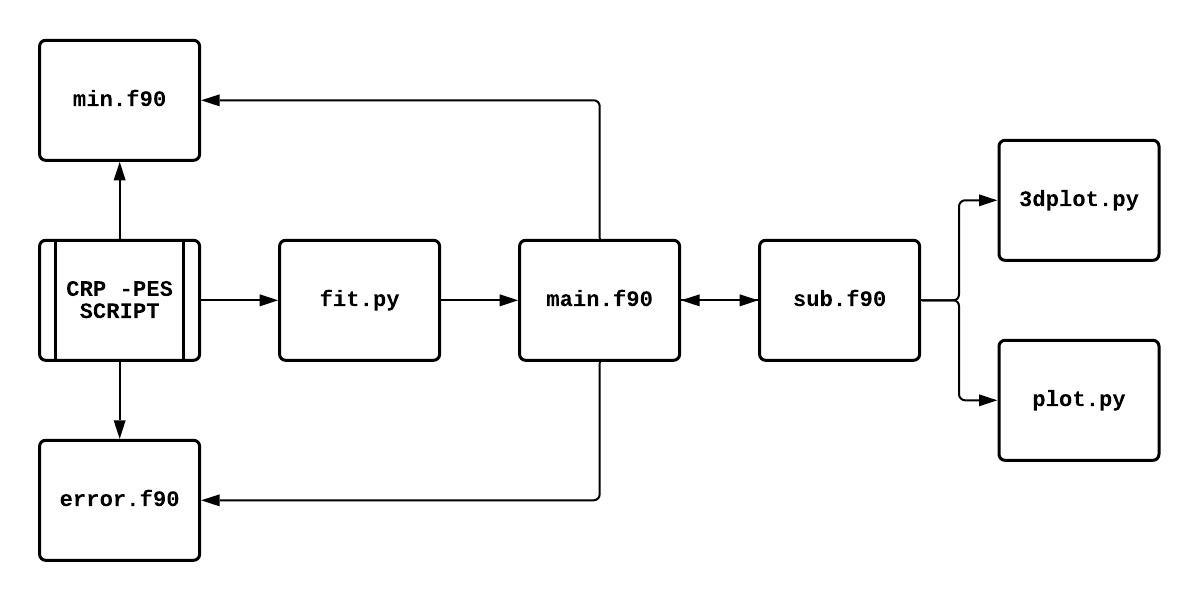
\includegraphics[width = \textwidth]{flow.jpeg}
    \caption{Information Diagram on flow of the program}
    \label{fig:1}
\end{figure}

\begin{figure}[h!]
    \centering
    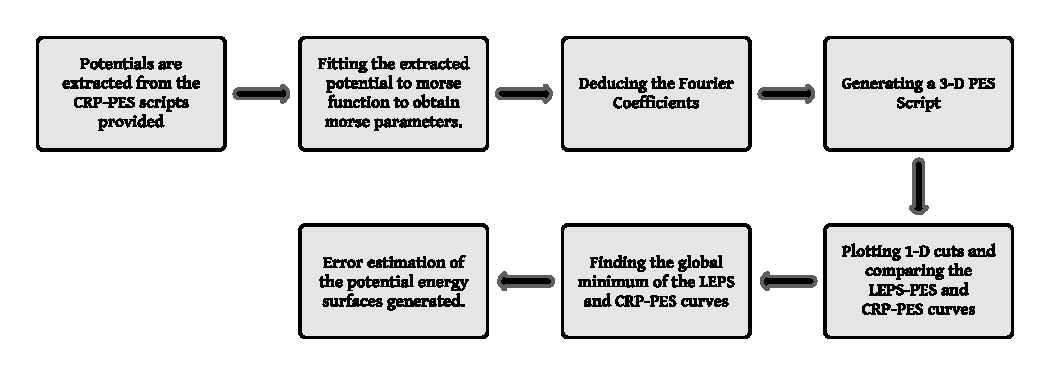
\includegraphics[width = \textwidth]{fndiag.pdf}
    \caption{Functional Diagram of the program} 
    \label{fig:2}
\end{figure}    

\section{RELIABILITY OF THE PROGRAM - QUALITY APPROACH}
\par\noindent\rule{\textwidth}{0.4pt}

\begin{enumerate}
    \item The LEPS potentials build by the program where compared to the CRP-PES obtained from the scripts that were provided. After the analysis of the results such as comparison of the LEPS and CRP-PES curves. It can be conculded that the program is reliable and can be used to produce LEPS potential energies that follow the trend of the CRP potential energies.
    \item For the curve fitting of the extracted CRP-PES potential energies, it  is important to have good initial parameters. These are however guesses and the curve fitting errors, if any, could be related to this problem.
    \item Moreover, we have also carried out a detailed error analysis of the obtained potential energies. The absolute error was found to be of an tolerable range. Whereas the relative error is dependent on the range of values on the z-axis over which the potential energies are extracted. For lesser error factors, the user should choose the range of z-axis closer to the potential well as the error factor increases as we move away from this region. This error optimization technique produces LEPS potential energies that are comparable to the CRP-PES potential energies
    \item The CPU run time was found to be very less in the order of milliseconds for the execution of the programs. Only the loading of large text files may cause a delay in the run time but this program was executed for total number of potential values in the range of N = 100-400. This execution did not produce any large text files and kept the CPU run time very low. The largest text file  was that of the two dimensional potential energies generated by the 3-D PES script and it was found to be in the order of 2 Megabytes. 
    \item For memory optimization, most arrays that have been defined are allocatable arrays that are not pre-defines memory spaces. Depending on the size of the text files, we allocate the memory to the arrays and after usage deallocate them 
    \item It is also possible to evaluate the CRP-PES for a larger number of potential energies. This would help in the optimization of the nonlinear curve fit that is produced.
    \item Following this, the LEPS potential energies that are build will also be at a large number of points and the potential energies evaluated at closer intervals would give lesser chances for the occurrence of errors.
    \item All the data that has been used for the execution of the program and and all the results obtained after the execution has been stored in the folder {\fontsize{10}{6}\code{files}}. These data can be extracted and used by the user to check for the reliability of this program.
    
\end{enumerate}

\section{OUTCOME EXAMPLES}
\par\noindent\rule{\textwidth}{0.4pt}

\subsection{CRP-PES}

The initial step of this project was to extract the potential energies from the provided CRP-PES scripts for various positions of N onto W(100) surfaces. The following 1-D cuts of the potential energy as a function of the N/W distance were obtained for the three high-symmetry sites; coordinates can be referred to in Table: \ref{f1}. These plots are made for a set of 300 points over the range of zmin = -2 \AA \hspace{0.5mm}  to zmax = 6 \AA. 

It can be noticed that the CRP-PES curves in figure: \ref{fig:2}  are like that of the Morse potential curves and hence we use the Morse function to model these curves in a non-linear curve fit. The 1-D cuts are plotted for the Bridge-1 and Bridge-2 coincide with each other and hence this can be chosen as a single high symmetry site - Bridge. 


\begin{figure}[h!]
    \centering
    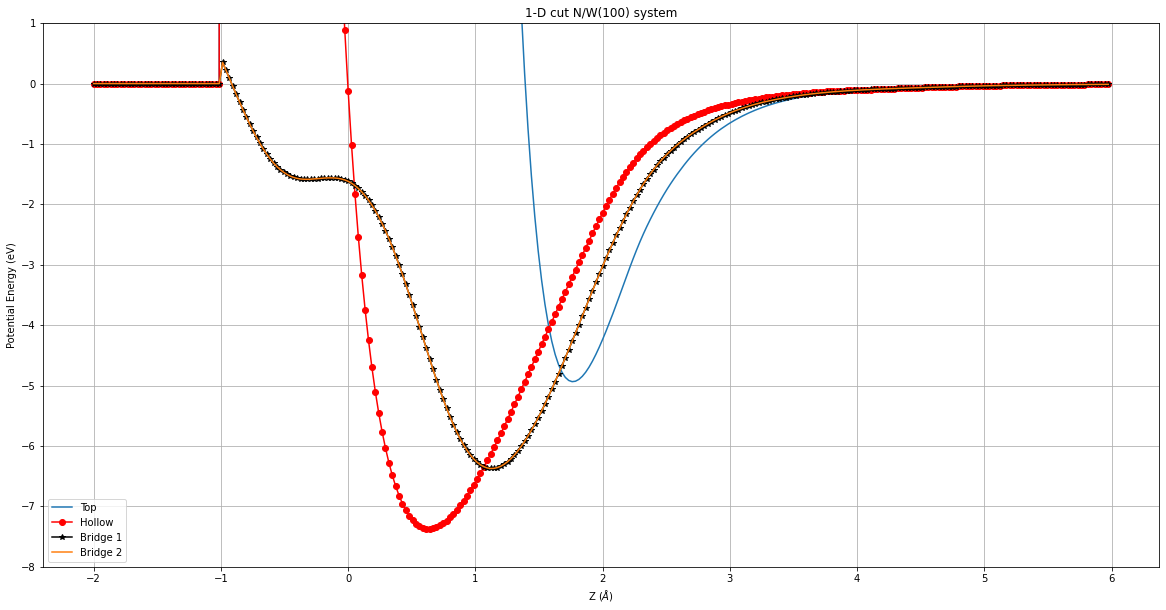
\includegraphics[scale = 0.35]{1Dcut.png}
    \caption{1-D cut: CRP-PES} 
    
    \label{fig:2}
\end{figure}   

\subsection{Non-linear Curve Fit}

\vspace{5mm}
In order to deduce the Fourier Coefficients, we need to obtain the Morse Potential Parameters. These parameters are obtained by performing a non-linear curve fit onto the CRP-PES curves with the Morse potential model. 

The initial parameters are set as:

\begin{enumerate}
    \item Initial Parameters for Top Symmetry\hspace{7mm}: [-8.0, 2.0, 3.0]
    \item Initial Parameters for Hollow Symmetry  : [-6.0, 1.0, 0.1]
    \item Initial Parameters for Bridge Symmetry\hspace{1.5mm}  : [-6.0, 1.0, 1.0]
\end{enumerate}
\vspace{5mm}

It was found that, when the range of the distances in the z-axis was takes to be negative, the Bridge and the Hollow symmetry showed unusual behaviour. It also made the modelling use the Morse function very difficult and hence these values were then excluded during the fitting procedure. Moreover, the behaviour of the high symmetry sites were such that they quickly approached extremely high potential energy values when the distance on the z-axis approached zero. These values once again, prevented np.polyfit from providing good fits for the plots. Hence, for the fitting procedure the range of distances in the z-axis was taken as zmin = 0.5 \AA \hspace{0.5mm} to zmax = 6-10 \AA. In this range we have removed the extremely fluctuating values of the potential to obtain a good fit.

\vspace{5mm}

We get the following values for the Morse Potential Parameters:

\begin{enumerate}
    \item Parameters for hollow symmetry are:  [7.60346595, 1.2495198,  0.56501317]
    \item Parameters for bridge symmetry are:  [6.55379066, 1.30169922, 0.95376732]
    \item Parameters for top symmetry are \hspace{4mm}: [4.9984788,  1.71646688, 1.83275503]
\end{enumerate}
\vspace{5mm}
The curve fit for each of the high symmetry sites - Top, Hollow and Bridge are given in the figures: \ref{fig:23}, \ref{fig:24} and \ref{fig:25}. We can conclude that the parameters obtained are good parameters by looking at the below fit. We see a fairly good coherence between the theoretical CRP potentials and the non-linear curves that have been fit.
\vspace{5mm}

The NumPy library makes use of numpy.polyfit() that carries out a Least-squares polynomial fit. However, this procedure doesn't necessarily have to be done using the pre-defined NumPy function. We could also manually write a FORTRAN or a Python code for the Least-Squares fit.

\begin{figure}[h!]
    \centering
    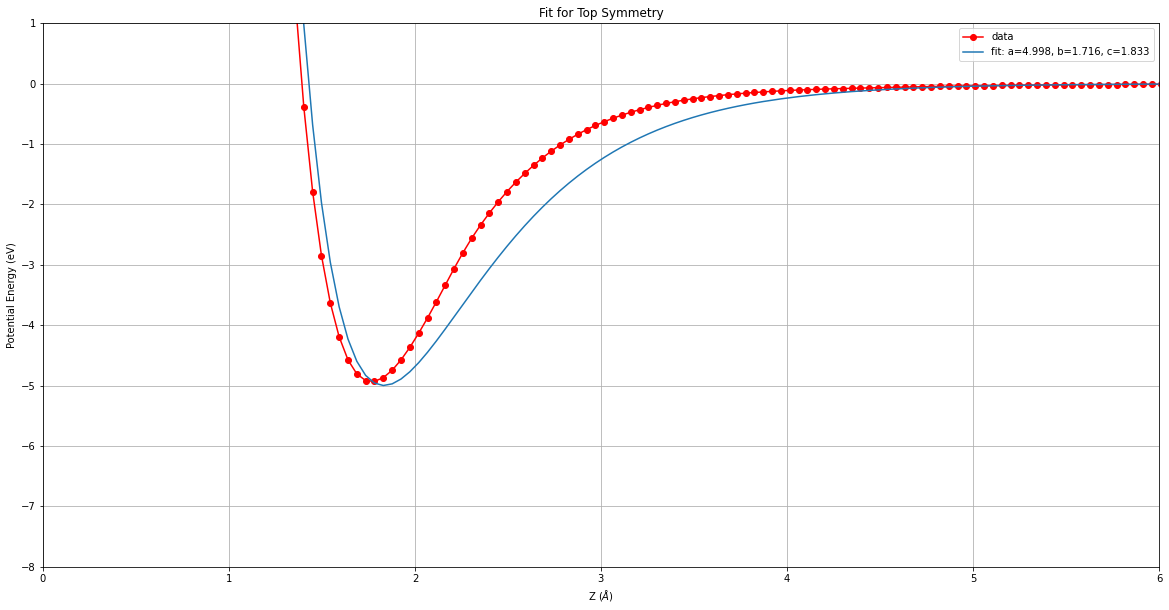
\includegraphics[scale = 0.28]{top.png}
    \caption{Non-linear curve fit for the High Symmetry Site - Top} 
    \label{fig:23}
\end{figure}  

\begin{figure}[h!]
    \centering
    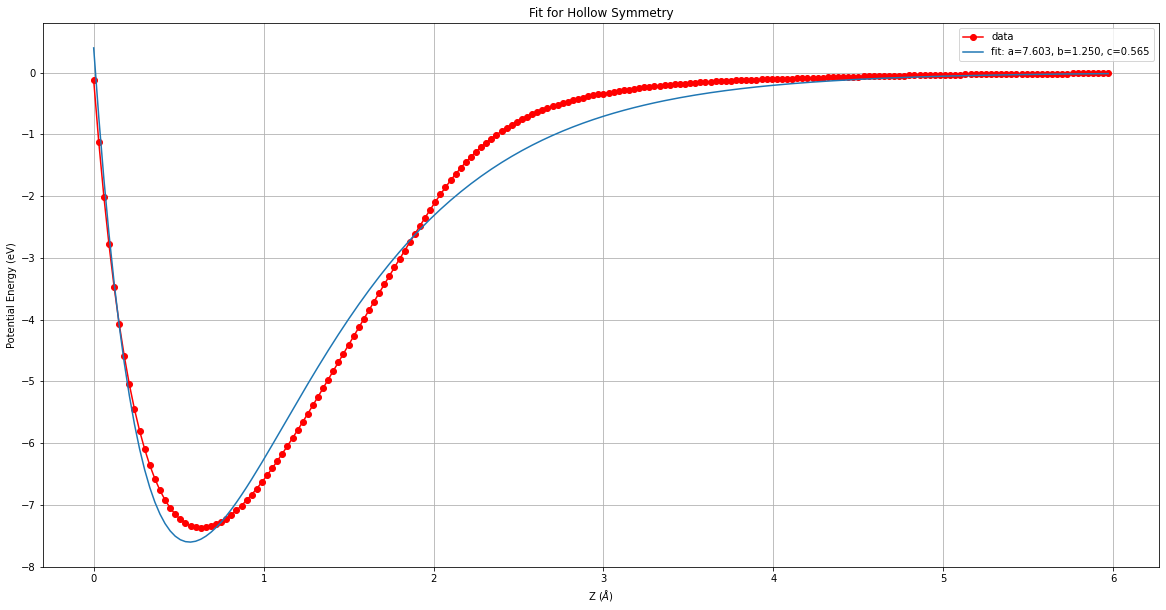
\includegraphics[scale = 0.28]{hollow.png}
    \caption{Non-linear curve fit for the High Symmetry Site - Hollow} 
    \label{fig:24}
\end{figure}  

\begin{figure}[h!]
    \centering
    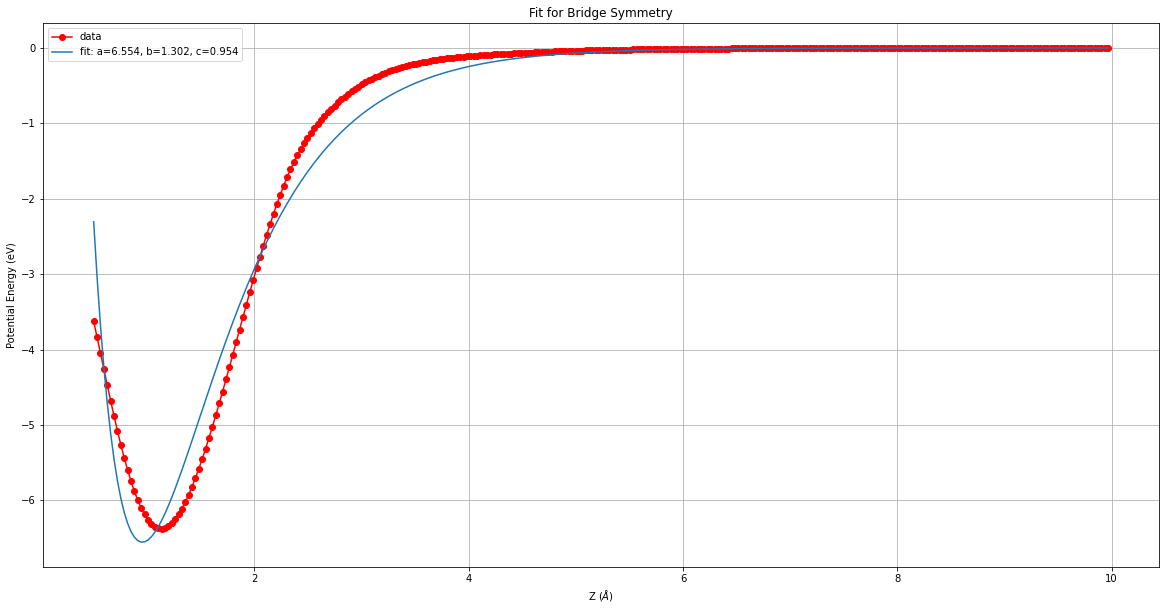
\includegraphics[scale = 0.28]{bridge.png}
      \caption{Non-linear curve fit for the High Symmetry Site - Bridge} 
    \label{fig:25}
\end{figure}  
\pagebreak
\subsection{Fourier Coefficients and Comparison of LEPS and CRP-PES curves}
\vspace{5mm}
Using the parameters obtained from the previous section, we were able to calculate the required Fourier Coefficients for each Morse Potential Parameter:

\begin{table*}[h!]\centering
\ra{1.3}
\resizebox{\linewidth}{!}{%
\begin{tabular}{cccc}\toprule
\textbf{Morse Potential Parameters}  & \textbf{First Fourier Coefficient $-P_0$} & \textbf{Second Fourier Coefficient - $P_1$} & \textbf{Third Fourier Coefficient - $P_3$}  \\\toprule
D & 8.9587 & -1.1614 & -0.8187 \\
$\alpha$ & 1.3979 & - 0.4278  & 0.5871  \\
$r^{eq}$  & 0.2568 & - 5.7649E-003 & 0.7938 \\
\hline
\end{tabular}}
\caption{Fourier Coefficients for the Morse Potential Parameters}
\label{t3}
\end{table*} 

From these Fourier Coefficients, we obtain the following plots for the three high symmetry sites (top, bridge, hollow) and for the
three lower symmetry sites (top-bridge, top-hollow, bridge-hollow). We also plot the comparison between the three HIGH symmetry sites in figure: \ref{fig:12} and the three LOW symmetry sites in the figure: \ref{fig:13}. Finally, we also provide a comparison of all the symmetry sites in the figure: \ref{fig:14}.
\vspace{5mm}
\begin{figure*}[h!]
    \centering
    \begin{subfigure}[t]{0.5\textwidth}
        \centering
            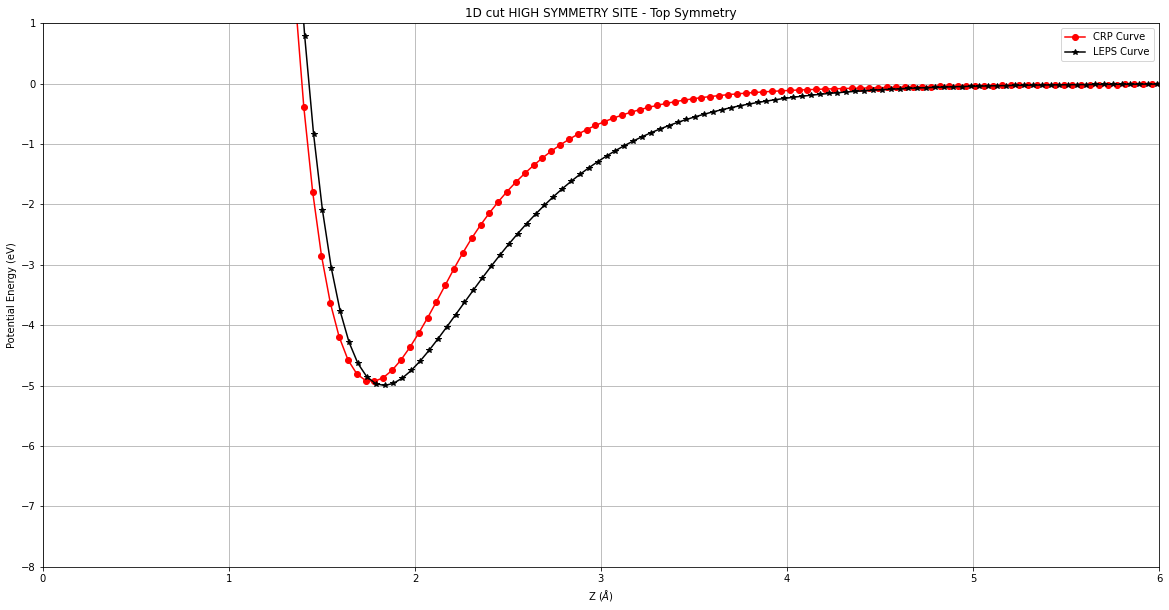
\includegraphics[scale = 0.2]{1dtop.png}
    \caption{1-D cut LEPS curve - Top} 
    \label{fig:6}
    \end{subfigure}%
    ~ 
    \begin{subfigure}[t]{0.5\textwidth}
        \centering
             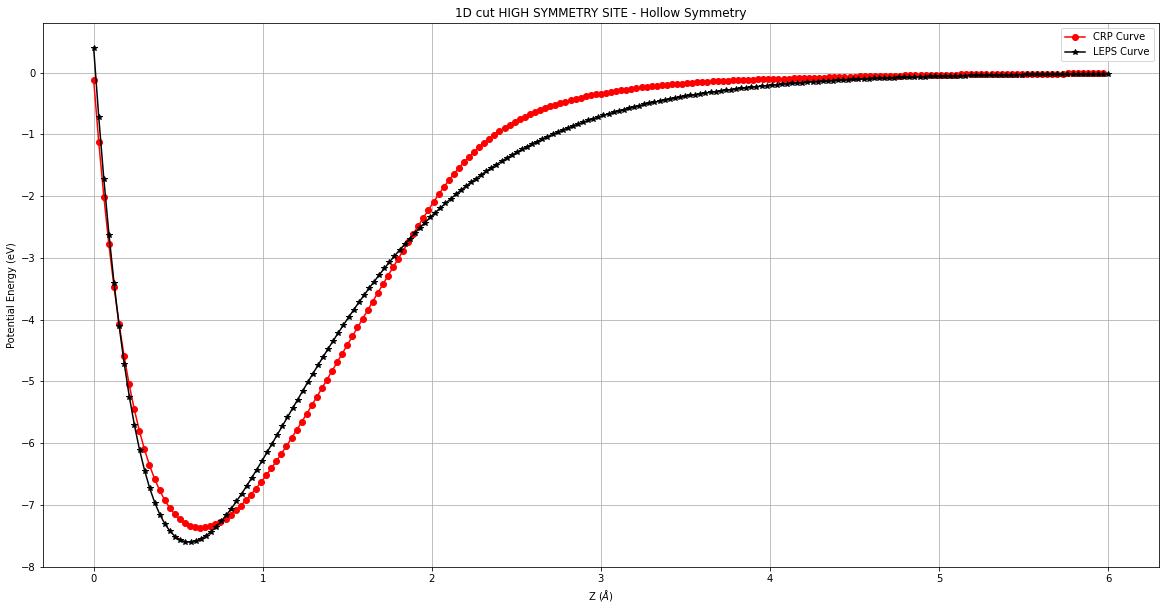
\includegraphics[scale = 0.2]{1dhollow.png}
    \caption{1-D cut LEPS curve - Hollow} 
    \label{fig:7}
    \end{subfigure}
\end{figure*}
\begin{figure*}[h!]
    \centering
    \begin{subfigure}[t]{0.5\textwidth}
        \centering
    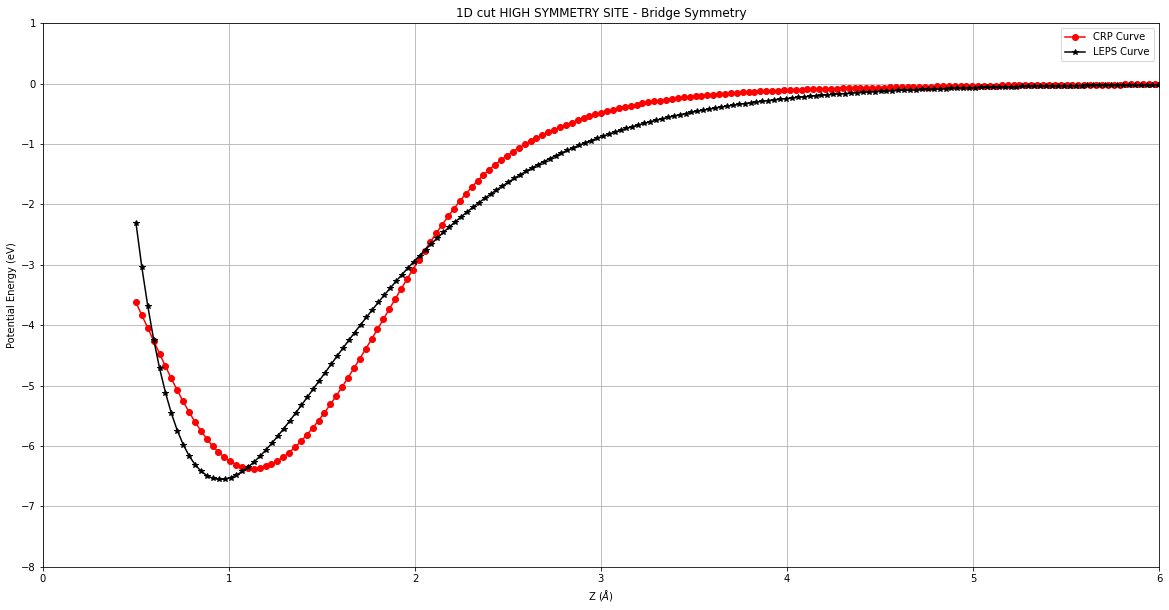
\includegraphics[scale = 0.2]{1dbridge.png}
      \caption{1-D cut LEPS curve - Bridge} 
    \label{fig:8}
    \end{subfigure}%
    ~ 
    \begin{subfigure}[t]{0.5\textwidth}
        \centering
    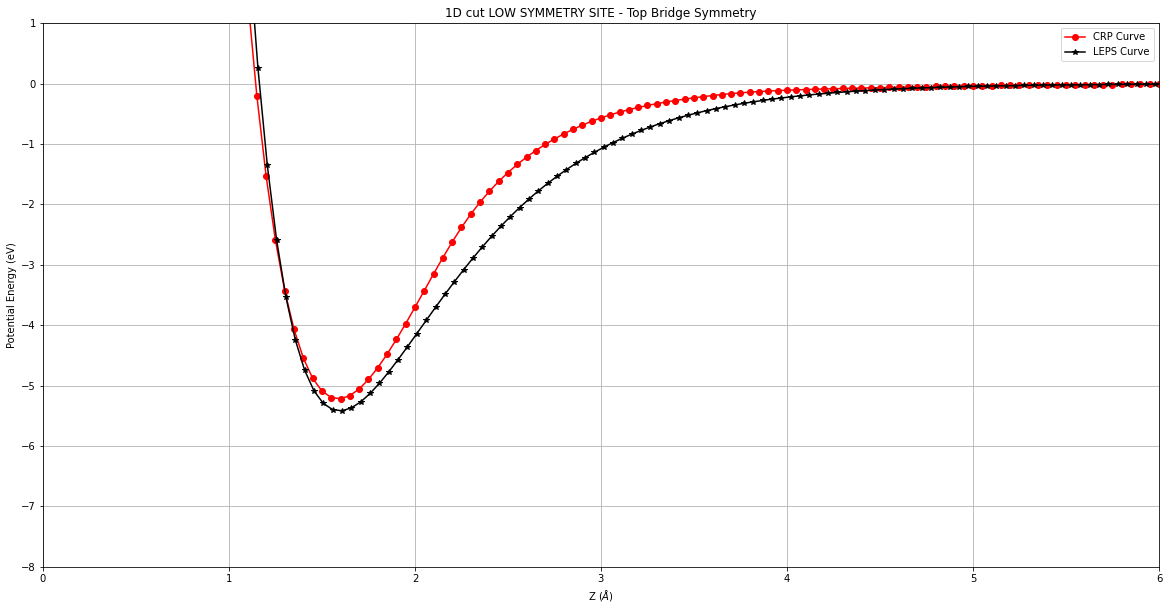
\includegraphics[scale = 0.2]{1dtopbridge.png}
    \caption{1-D cut LEPS curve - Top Bridge} 
    \label{fig:9}
    \end{subfigure}
    
\end{figure*}

\begin{figure*}[h!]
    \centering
    \begin{subfigure}[t]{0.5\textwidth}
        \centering
               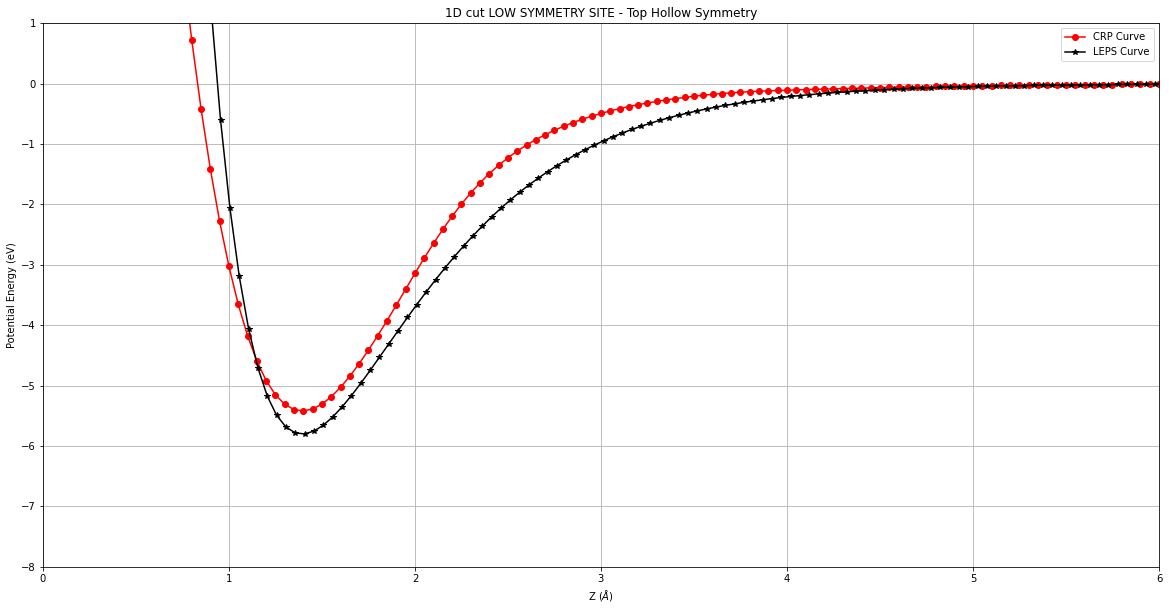
\includegraphics[scale = 0.2]{1dtophollow.png}
    \caption{1-D cut LEPS curve - Top Hollow} 
    \label{fig:10}
    \end{subfigure}%
    ~ 
    \begin{subfigure}[t]{0.5\textwidth}
        \centering
    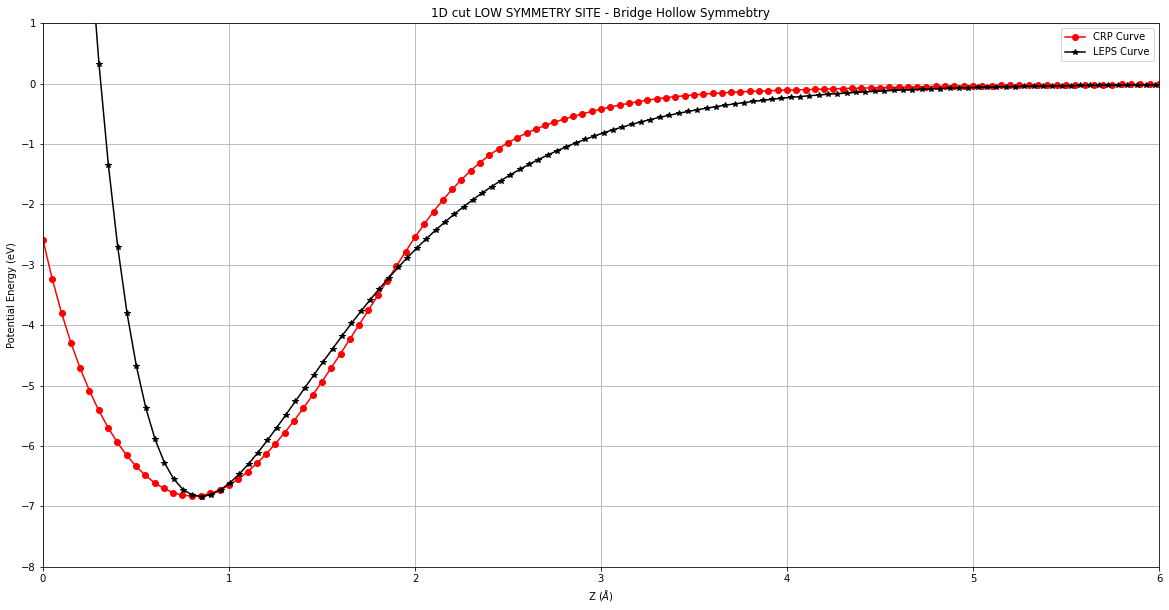
\includegraphics[scale = 0.2]{1dbridgehollow.png}
      \caption{1-D cut LEPS curve - Bridge Hollow} 
    \label{fig:11}
    \end{subfigure}
\end{figure*}
\begin{figure*}[h!]
    \centering
    \begin{subfigure}[t]{0.5\textwidth}
        \centering
    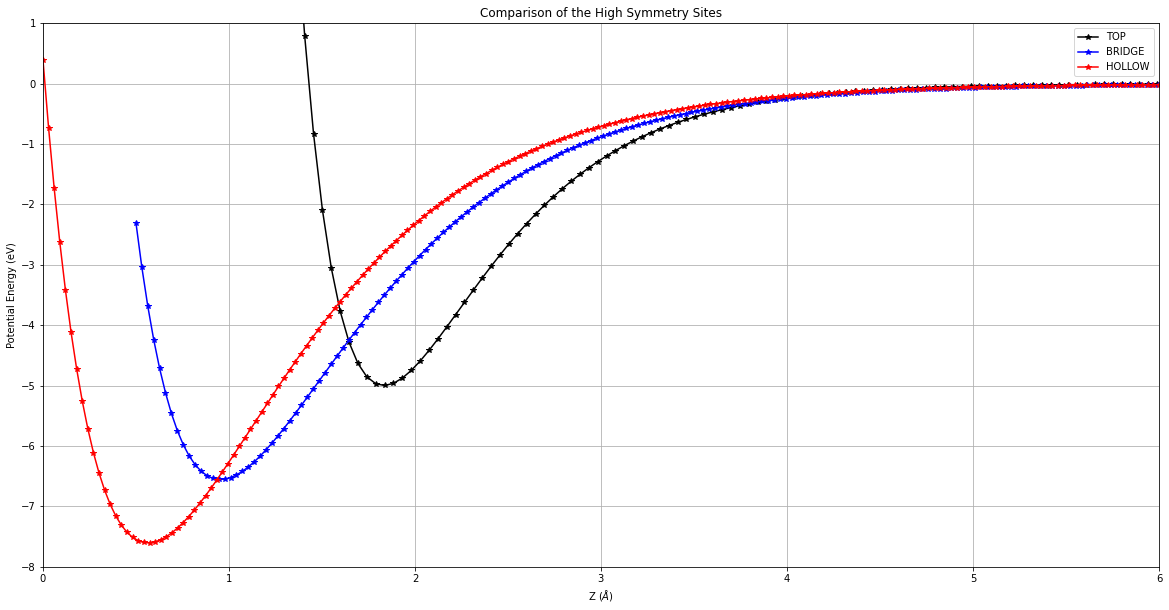
\includegraphics[scale = 0.2]{comprisonhigh.png}
      \caption{1-D cut LEPS curve - High symmetry sites} 
    \label{fig:12}
    \end{subfigure}%
    ~ 
    \begin{subfigure}[t]{0.5\textwidth}
        \centering
    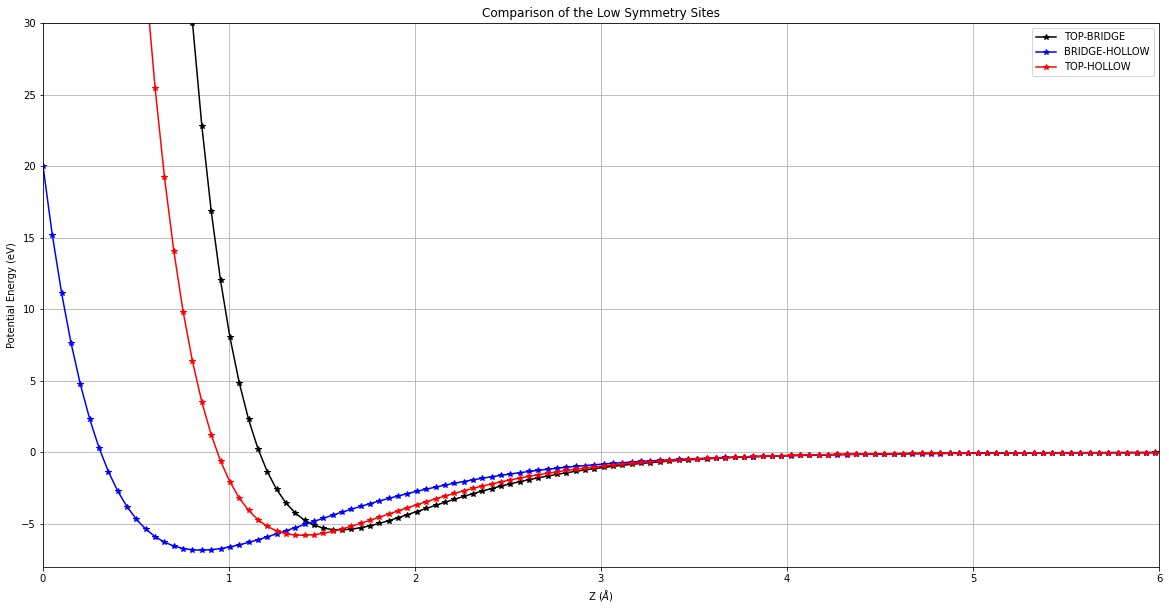
\includegraphics[scale = 0.2]{comparisonlow.png}
    \caption{1-D cut LEPS curve -Low symmetry sites} 
    \label{fig:13}
    \end{subfigure}
    \caption{Comparison of LEPS and CRP-PES curves}
\end{figure*}
    
\begin{figure}[h!]
    \centering
    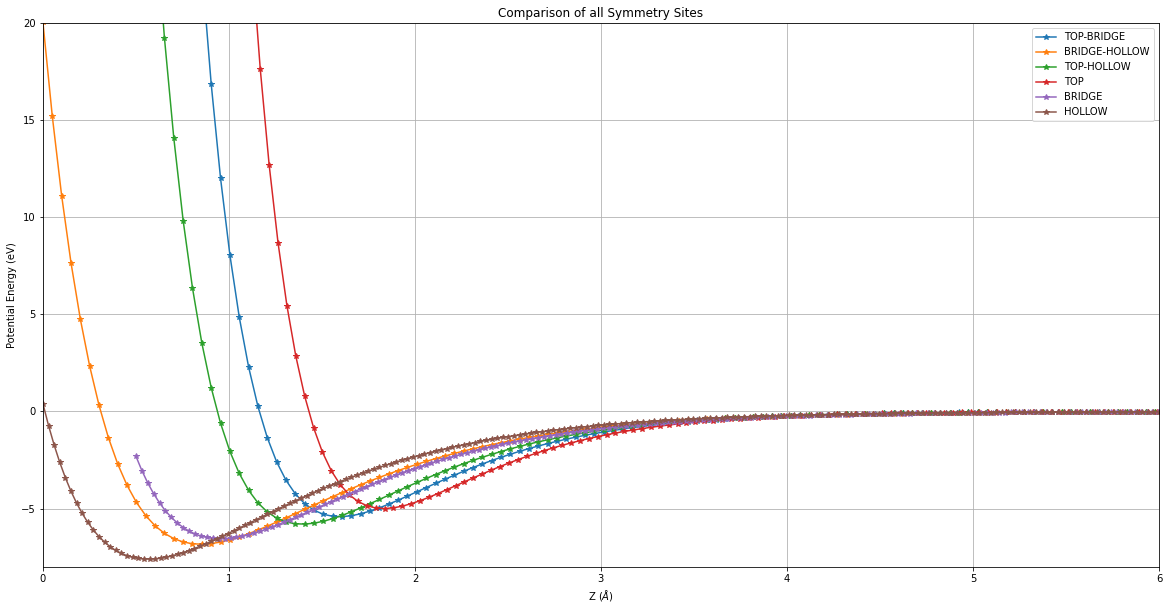
\includegraphics[scale = 0.28]{comparison.png}
      \caption{Comparison of all the symmetry sites} 
    \label{fig:14}
\end{figure}  

\pagebreak
\subsection{Testing of the 3-D PES Script}

The 3D PES script generated by making the following three dimensional plots from the two dimensional potential plotted against the range of values on the y-axis and z-axis for a fixed x-value. 

In this program, the 3-D scripts are done for a fixed point on the x-axis and a range of values on the y and z-axis. However with slight modification to the program, it is possible to generate these scripts for fixed points on y and z-axis and evaluating the potential energies over the other two axis.

The plot generated in figure: \ref{fig:35} shows the behaviour of a Morse function with a depth D around -6 eV and the potential increasing as z reached zero. Hence, the nature of the 3D-PES script has been tested and it is believed to be accurate from the obtained results.
    
\begin{figure}[h!]
    \centering
    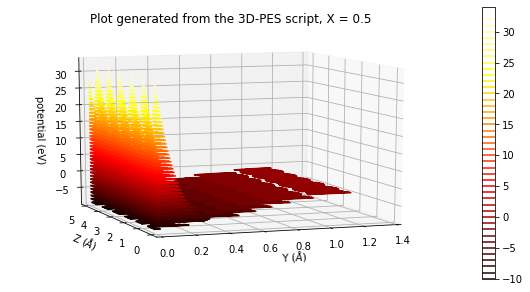
\includegraphics[width = \textwidth]{3d.png}
      \caption{Plot generated from the 3D-PES script for X=0.5\AA} 
    \label{fig:35}
\end{figure}     

\subsection{Global Minimum}
\vspace{5mm}
On the comparison of all the minimum values of the LEPS and CRP-PES curves, we were able to find the Global minimum for these two curves for the atom/surface by associating the
energy barrier to reach this energy minimum. We have the following results
\vspace{5mm}
\begin{center}
    The Global minimum for the \textbf{CRP}  - Potential Energy Surfaces: -7.37103987 eV
  
    The Global minimum for the \textbf{LEPS} - Potential Energy Surfaces: -7.60317278 eV
\end{center}

\subsection{Error analysis}
\vspace{5mm}
Due to the nature of the Morse function, it is not possible to directly calculate the mean error, instead we find the deviation of each LEPS potential energy from that of the CRP potential energies. The error is calculated for each point after which a mean error is calculated. We get the following results - 

\vspace{5mm}
\begin{center}
      
  \textbf{Mean absolute error} for High Symmetry Site: \textbf{Hollow} -   0.212
  
  \textbf{Mean relative error} for High Symmetry Site: \textbf{Hollow} -    53.927\% 
  
  \vspace{5mm}
  
  \textbf{Mean absolute error} for High Symmetry Site: \textbf{Bridge} -   0.148     
  
 \textbf{ Mean relative error} for High Symmetry Site: \textbf{Bridge} -    235.399\% 
  
  \vspace{5mm}
  
  \textbf{Mean absolute error} for High Symmetry Site: \textbf{Top} -   0.324
  
 \textbf{ Mean relative error} for High Symmetry Site:\textbf{ Top} -    78.009\%
  
  \vspace{5mm}
  
  \textbf{Mean absolute error} for Low Symmetry Site: \textbf{Top Bridge} -  15.347   
  
  \textbf{Mean relative error} for Low Symmetry Site: \textbf{Top Bridge} - 115.161\%
  
  \vspace{5mm}
  
  
  \textbf{Mean absolute error} for Low Symmetry Site: \textbf{Top Hollow} - 7.359  
  
  \textbf{Mean relative error} for Low Symmetry Site:\textbf{ Top Hollow }- 162.949\%
  
  \vspace{5mm}
  
  
  \textbf{Mean absolute error} for Low Symmetry Site: \textbf{Bridge Hollow} - 0.627
  
  \textbf{Mean relative error} for Low Symmetry Site: \textbf{Bridge Hollow }- 254.640\%
  

\end{center}
\vspace{5mm}
The error factor received from the Relative error calculation was huge even though the fit produces looked coherent. After several tries to debug the code and thorough analysis of the potential energies studied, it was realised that the huge error factor was result of the long range of distances in the z-axis. As the z axis extended beyond 6-7 \AA, it was found that the error between the CRP potential and LEPS potential points increased drastically. However, this is not visible on the plots due to extremely small values of potentials in this region. This hypothesis was rechecked by running an error analysis on the potentials in the range 0.5-7 \AA. We obtain the following results:
\begin{figure}[h!]
    \centering
    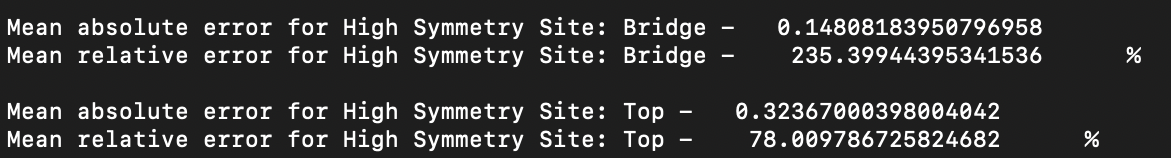
\includegraphics[width = \textwidth]{errorbefore.png}
      \caption{Error analysis for z - 0.5 to 10\AA} 
    \label{fig:38}
\end{figure}     
\begin{figure}[h!]
    \centering
    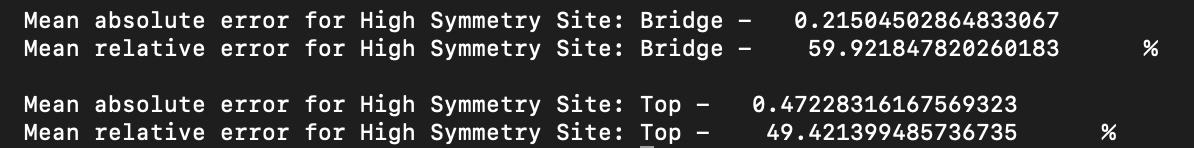
\includegraphics[width = \textwidth]{errorafter.png}
      \caption{Error analysis for z - 0.5 to 7\AA} 
    \label{fig:39}
\end{figure}     

On comparison of the two figures:\ref{fig:38} and \ref{fig:39} , one can see the drastic decrease in the values of the Relative errors. The relative error for the High symmetry site - bridge drops from 235\% to just around 60\%. Similarly there is also a drop in the error percentage of the High Symmetry site - Top. This decrease in the error factor was verified for all symmetry sites and hence it can be concluded that the range at which the LEPS potential energies are evaluated, play an important role in the reduction of error.

\section{CONCLUSION}
\par\noindent\rule{\textwidth}{0.4pt}

The main objective of this project was to develop a simplified three dimensional potential to describe the N/W(100) interactions. We were able to obtain LEPS potential values that showed good coherence to the provided CRP potentials. The plot of the three dimensional potential surface also portrays a Morse function which is in correspondence to the model that was used to build the LEPS potentials. Even though, there are some abnormalities in the mean relative errors, we have obtained tolerable absolute errors that verifies the reliability of the program developed. This project could have been further developed to represent the modified Morse potential by obtaining the eight Morse potential parameters. However, due to time constraints and some lack of clarity in the first few parts of the project, this was not achieved.



\end{document}
